\section{Polynomial expected depth with two modified initial budgets}
\label{sec:two-phase}

The same idea can modify the second budget as well as the first.
This gives a deterministic polynomial-time expected-depth factor
below $5.182976$ under arbitrary strictly positive rational priors.
The gain comes from moving the second coverage batch slightly earlier
or later, while preserving its exact coverage guarantee. Discovery
modes, endpoint recovery, and the recursive potential are unchanged.

\subsection{The actual schedule family}

Set
\begin{equation}\label{eq:two-phase-parameters}
 \beta=\frac{3512863}{10^6},\qquad
 \delta=\frac{393931}{2500000}=0.1575724.
\end{equation}
For a rational shift representative $u$, write
$k_j=\lfloor\beta^ju\rfloor$. In addition to all initial variants of
Algorithm~\ref{alg:first-phase-family}, try
\[
 \begin{array}{ll}
 q,r,k_2,k_3,\ldots,
 &1\le q\le6,\quad r\in\{k_1-1,k_1,k_1+1\},\quad q<r<k_2,\\
 q,k_2,k_3,\ldots,&1\le q\le6.
 \end{array}
\]
The second line omits the original second phase. At every executed
budget $k$, use the exact maximum-coverage set $Q_k$ if
$k<k_{\min}$; otherwise use the minimum cover $Q_*$ and finish.
Within a batch, append productive unused blocks greedily by newly
covered mass. Choose adaptive modes by Algorithm~\ref{alg:block-mode}
and minimize the same rational score
\[
 F_*(G)=2\MSSC_{\rm blk}(G)+2p_0|G|-\operatorname{Save}(G).
\]
Thus the new family retains every earlier initial schedule at a fixed
state. Its new balance threshold is used at every recursive state.
The proof needs only the displayed two-budget subfamily.

\begin{algorithm}[H]
\caption{Two modified initial budgets for \ExpectedTree}
\label{alg:two-phase-family}
\KwIn{Positive-pattern block demands and weights; zero weight $p_0$;
parameters of \eqref{eq:two-phase-parameters}.}
\KwOut{A minimum rational-score candidate schedule.}
Reuse the coverage sets $Q_k$ and minimum cover $Q_*$\;
Refine the \BatchOrders\ shift partition by
\eqref{eq:initial-shift-refinement}; use its breakpoints and cell midpoints\;
Retain the best initial-batch candidate of
Algorithm~\ref{alg:first-phase-family}, using the current state and $\delta$\;
\ForEach{shift representative $u$}{
 $k_1\gets\lfloor\beta u\rfloor$;
 $k_2\gets\lfloor\beta^2u\rfloor$\;
 \For{$q=1,\ldots,6$}{
  $\mathcal V\gets\{(q,0)\}\cup
   \{(q,r):r\in\{k_1-1,k_1,k_1+1\},\ q<r<k_2\}$\;
  \ForEach{$(q,r)\in\mathcal V$}{
   $G\gets$ empty order\;
   Process budgets $q$, then $r$ if $r>0$, then
   $\lfloor\beta^ju\rfloor$ for $j=2,3,\ldots$\;
   At each budget $k$, greedily append productive unused blocks
   of $Q_k$ if $k<k_{\min}$, and of $Q_*$ otherwise\;
   Stop these phases once $k\ge k_{\min}$\;
   Use Algorithm~\ref{alg:block-mode} to compute rational savings $D$\;
   Retain $G$ with score
   $2\MSSC_{\rm blk}(G)+2p_0|G|-\sum D$\;
  }
 }
}
\KwRet a retained schedule of minimum score\;
\end{algorithm}

There are at most twenty-four new variants per shift representative.
The refinement \eqref{eq:initial-shift-refinement} adds a constant
number of cells for fixed $\beta$ and explicitly includes all
initial breakpoints, even when $k_{\min}$ is small. This matters
for $r=k_1-1$: its change from a partial batch to a complete cover
can occur at $k_1=k_{\min}+1$, beyond the truncated base partition.
All later executed-budget breakpoints belong to the base partition.
Hence the actual schedule and rational score are constant on every
refined cell, and every shift used by the forty-three-row proof
distribution is represented by an actual candidate. Neither logarithms
nor the proof distribution are evaluated by the algorithm.
Use Algorithm~\ref{alg:two-phase-family} for flat-state scheduling
in the adaptive variant of \ExpectedTree. Singleton and degenerate-hull
cases use the existing direct procedures.

\begin{figure}[htbp]
\centering
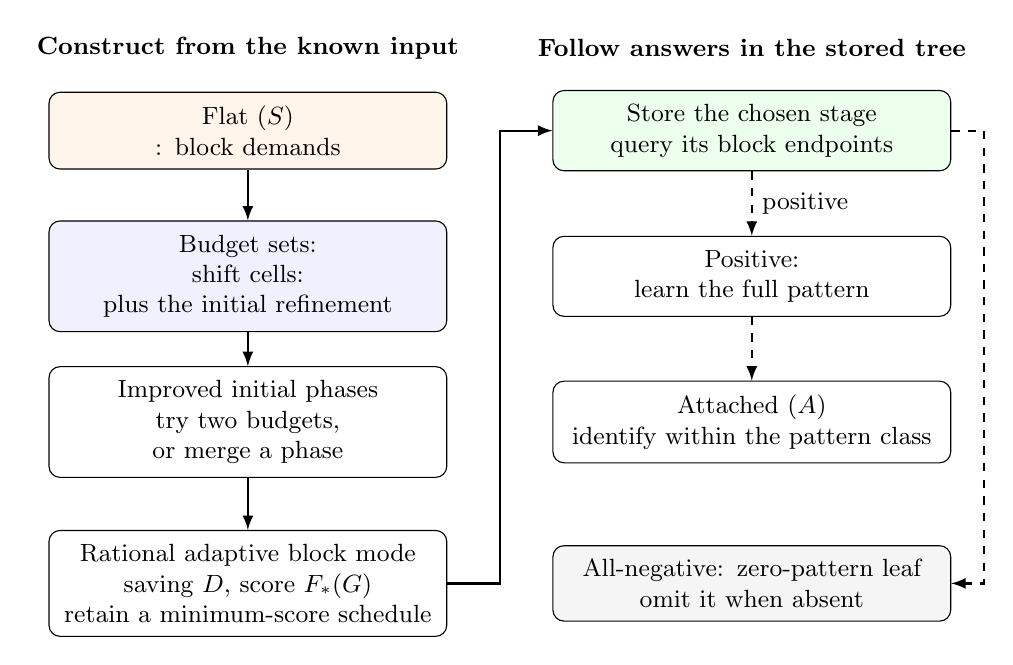
\begin{tikzpicture}[every node/.style={font=\small},
  box/.style={draw,rounded corners,align=center,inner sep=5pt,text width=4.7cm},
  arr/.style={-latex,thick},exec/.style={-latex,thick,dashed}]
  \node[font=\small\bfseries] at (-3.2,1.05) {Construct from the known input};
  \node[font=\small\bfseries] at (3.2,1.05) {Follow answers in the stored tree};
  \node[box,fill=orange!8] (hull) at (-3.2,0)
    {Flat \ExpectedTree$(S)$\\\HullData: block demands};
  \node[box,fill=blue!6] (covers) at (-3.2,-1.85)
    {Budget sets: \IntervalCover\\shift cells: \BatchOrders\\plus the initial refinement};
  \node[box] (variants) at (-3.2,-3.7)
    {Improved initial phases\\try two budgets, or merge a phase};
  \node[box] (score) at (-3.2,-5.75)
    {Rational adaptive block mode\\saving $D$, score $F_*(G)$\\retain a minimum-score schedule};
  \node[box,fill=green!7] (stored) at (3.2,0)
    {Store the chosen stage\\query its block endpoints};
  \node[box] (positive) at (3.2,-1.85)
    {Positive: \EndpointCode\\learn the full pattern};
  \node[box] (child) at (3.2,-3.7)
    {Attached \ExpectedTree$(A)$\\identify within the pattern class};
  \node[box,fill=gray!8] (zero) at (3.2,-5.75)
    {All-negative: zero-pattern leaf\\omit it when absent};
  \draw[arr] (hull) -- (covers);
  \draw[arr] (covers) -- (variants);
  \draw[arr] (variants) -- (score);
  \draw[arr] (score.east) -- (0,-5.75) -- (0,0) -- (stored.west);
  \draw[exec] (stored) -- node[right]{positive} (positive);
  \draw[exec] (positive) -- (child);
  \draw[exec] (stored.east) -- (6.15,0) -- (6.15,-5.75)
    -- (zero.east);
\end{tikzpicture}
\caption{The improved polynomial expected-depth procedure, including
the two-budget family of Algorithm~\ref{alg:two-phase-family}. The shift
cells include the refinement \eqref{eq:initial-shift-refinement}. Solid
arrows are construction-time data flow, computed from the supplied incidence
table and rational priors. Dashed arrows show how the unknown hypothesis
traverses the resulting tree; endpoint decoders and recursive children
are already constructed. Adaptive modes choose whether the first
positive block stops early or queries both endpoints. The certificate's
mixture is used in the proof of the bound, not to randomize execution.}
\label{fig:expected-procedure-flow}
\end{figure}



\subsection{One signed correction for each affected cost}

The unaveraged first-hit upper bound for the two-budget variant is
\[
 \begin{aligned}
 \phi_{u,q,r}(t)={}&\frac{q+1}{2}
  +\frac{q+r}{2}\mathbf1_{\{t>q\}}
  +\frac{r+k_2}{2}\mathbf1_{\{t>r\}}\\
 &+\frac12\sum_{j\ge2}(k_j+k_{j+1})\mathbf1_{\{t>k_j\}}.
 \end{aligned}
\]
For the one-budget variant, replace the two initial transition terms
by $(q+k_2)\mathbf1_{\{t>q\}}/2$.
Subtracting either bound from the old $\phi_u(t)$ gives the exact
doubled improvement
\begin{equation}\label{eq:two-phase-correction}
 \begin{aligned}
 d_{q,r}(u,t)={}&k_0-q+(k_0+k_1)\mathbf1_{\{t>k_0\}}
               +(k_1+k_2)\mathbf1_{\{t>k_1\}}\\
 &-(q+r)\mathbf1_{\{t>q\}}-(r+k_2)\mathbf1_{\{t>r\}},
       &&r>0,\\
 d_{q,0}(u,t)={}&k_0-q+(k_0+k_1)\mathbf1_{\{t>k_0\}}
               +(k_1+k_2)\mathbf1_{\{t>k_1\}}\\
 &-(q+k_2)\mathbf1_{\{t>q\}}.
 \end{aligned}
\end{equation}
The signs matter: changing a budget can delay some witness ranks.
Every modified budget sequence is strictly increasing, so its
first-hit upper bound is nondecreasing. An earlier actual comparison
hit therefore improves the bound. The within-batch proof of
Lemma~\ref{lem:mssc} applies to each sequence; early completion at
$Q_*$ only removes nonnegative residual terms.

The all-negative route has a different invoice. With $k=k_{\min}$,
its length change relative to the old unrolled budget sum is
\begin{equation}\label{eq:two-phase-zero-correction}
 z_{q,r}(u,k)=q\mathbf1_{\{q<k\}}+r\mathbf1_{\{r<k\}}
             -k_0\mathbf1_{\{k_0<k\}}
             -k_1\mathbf1_{\{k_1<k\}},
\end{equation}
where the $r$ term is zero for the one-budget variant.
This prices the complete negative route, rather than only the first
positive hit.

\subsection{A finite certificate and the common ledger}

Retain the witness masses $m_t$, prefix masses $M_q$, and discounts
$e_\beta(t)$ from Section~\ref{sec:polynomial-blocks}. Exact coverage
makes the first batch cover at least $M_q$ with at most $q$ blocks.
Its total adaptive-mode saving is therefore at least each of
\[
 \mathsf A_q=M_q-\delta wq,\qquad
 \mathsf C_q=c_*M_q-d_*\delta wq,\qquad 0,
\]
by Lemma~\ref{lem:affine-block-credit}. These remain valid if the first
batch completes the minimum cover. Later savings are nonnegative.

Section~\ref{sec:two-phase-certificate} gives a fixed rational
forty-three-row distribution of variants and first-batch minorants.
The shift is log-uniform, and each row has constant $k_0,k_1,k_2$.
For a row $[l,h)$ of probability $P=\ln(h/l)/\ln\beta$, an option
of conditional weight $v$ and minorant $sM_q-\rho\delta w$ contributes
\begin{equation}\label{eq:two-phase-coefficients}
 a_t\gets a_t+Pv\bigl[d_{q,r}(u,t)+s\mathbf1_{\{t\le q\}}\bigr],
 \qquad \mu\gets\mu+Pv\rho,
\end{equation}
starting with $a_t=e_\beta(t)$ and $\mu=0$.
This is a joint comparison of the actual schedule's signed first-hit
change and its actual saving:
\[
 \sum_t m_t e_\beta(t)+
 \mathbb E\left[\sum_t m_t d_{q,r}(u,t)
                     +\operatorname{Save}(G)\right]
 \ge\sum_t m_t a_t-\delta w\mu.
\]
No comparison rank is identified with an actual discovery rank, and
no saving is counted twice.

Take $\tau=2190079/10^6=2.190079$ and set
\begin{equation}\label{eq:two-phase-chi-B}
 \chi=\tau-2\delta(\tau-a_1)-\delta\mu,\qquad
 B=7-\frac{\ln6}{\ln\beta}-\chi.
\end{equation}
Exact outward logarithm enclosures give
\[
 \begin{aligned}
 1.276476788627&<a_1<1.276476788629<\tau,\\
 \min_{2\le t\le14}a_t&>2.1900797161>\tau,\\
 4.461183727318&<\mu<4.461183727321,\\
 1.199202587061&<\chi<1.199202587065,\\
 4.374727111309&<B<4.374727111314.
 \end{aligned}
\]
All saving cutoffs are at most six, $k_0\le3$, $k_1\le12$, and
$r\le13$. Hence every signed correction is constant for $t\ge14$.
For one constant $\kappa$, $a_t=e_\beta(t)+\kappa$ on that entire
tail; monotonicity of $e_\beta$ reduces it to the $a_{14}$ check.
Only $a_1$ lies below $\tau$.

Let $D_0(k)=\mathbb E[z_{q,r}(u,k)]$. The same certificate gives
$D_0(1)=0$ and, for $k=2,\ldots,14$ in that order,
\[
 \begin{split}
 D_0(k)<{}&-.24607,\ -.30801,\ -.33917,\ -.31328,
            \ -.26141,\ -.21949,\ -.18652,\\
          &-.15871,\ -.13510,\ -.11546,\ -.09779,
            \ -.08368,\ -.06992.
 \end{split}
\]
For $k\ge14$, $D_0(k)=D_0(14)$, since all affected budgets are at
most thirteen. Thus the full mean waiting length still satisfies
$\mathbb E[|G|]\le Z_\beta(k_{\min})$ for every cover size. The
supporting witness and $\lambda_\beta>\nu_\beta$ retain the original
zero-route credit $2p_0/\ln\beta$.

Finally, the certificate gives $\chi+2/\ln\beta>\tau$.
Lemma~\ref{lem:capped-rank-credit} applies with $E=\{1\}$ and
$\zeta=2/\ln\beta$, converting all these terms into the saving
$\chi b$. Choosing the minimum rational score costs at most averaging
that score over the fixed distribution. Substitution into
\eqref{eq:adaptive-stage} yields the same local ledger as before:
\begin{equation}\label{eq:two-phase-local}
 W_{\rm pat}(S)\le A\Delta+B b+\frac{I-J_*}{\ln2},
 \qquad A=\frac{\beta+1}{\ln\beta}.
\end{equation}
The degenerate hull also satisfies this bound because $A,B>2$.

\begin{theorem}[Two-initial-budget polynomial approximation]
\label{thm:two-phase-expected}
For general supplied binary unit-cost planar line queries and arbitrary
strictly positive rational priors, the two-initial-budget adaptive
algorithm runs in deterministic polynomial time and has factor
\[
 \boxed{\rho_{\rm two}=
 A+\max\{\ln2/h(\delta),\ B\ln2/\sigma(\delta)\}<5.182976.}
\]
Its running-time exponent has no dependence on the smallest prior.
\end{theorem}
\begin{proof}
Apply Lemma~\ref{lem:stage-conversion} to
\eqref{eq:two-phase-local} and \eqref{eq:coarse-discovery-cap}.
Here $6<1/\delta<7$, so
$\sigma(\delta)=-6\delta\ln\delta
 -(1-6\delta)\ln(1-6\delta)$.
The rational logarithm bounds \eqref{eq:rational-log-bounds} certify
all comparisons above and
\[
 A+\max\{\ln2/h(\delta),B\ln2/\sigma(\delta)\}
 <5.182975508794<5.182976.
\]
The reproducible certificate \texttt{expected-two-phase-check.py}
also verifies $\lambda_\beta>\nu_\beta$, the accepted entropy tent,
$9{,}900$ exact signed-phase identities, and $1{,}650$ finite modified
batch comparisons including early completion and negative-route
lengths. The proof uses the fixed rational data of
Section~\ref{sec:two-phase-certificate}; it has no floating-point
optimization assumption.

The family adds a constant number of candidates per polynomial shift
partition. Coverage DPs, mode scores, and all decisions remain
rational and polynomial; the full-pattern recursive classes remain
disjoint proper subsets. Every actual query is a supplied endpoint
line. The singleton and degenerate-hull procedures retain their
existing guarantees.
\end{proof}
